\documentclass[letterpaper,10pt,onecolumn]{article}
\usepackage[spanish]{babel}
\usepackage[latin1]{inputenc}
\usepackage{amsfonts}
\usepackage{amsthm}
\usepackage{amsmath}
\usepackage{mathrsfs}
\usepackage{empheq}
\usepackage{enumitem}
\usepackage[pdftex]{color,graphicx}
\usepackage{hyperref}
\usepackage{listings}
\usepackage{calligra}
\usepackage{algpseudocode} 
\DeclareMathAlphabet{\mathcalligra}{T1}{calligra}{m}{n}
\DeclareFontShape{T1}{calligra}{m}{n}{<->s*[2.2]callig15}{}
\newcommand{\scripty}[1]{\ensuremath{\mathcalligra{#1}}}
\lstloadlanguages{[5.2]Mathematica}
\setlength{\oddsidemargin}{0cm}
\setlength{\textwidth}{490pt}
\setlength{\textheight}{610pt}
\setlength{\topmargin}{-85pt}
\addtolength{\hoffset}{-0.3cm}
\addtolength{\textheight}{4cm}

\begin{document}
\thispagestyle{empty}
\begin{center}


\includegraphics[width=490pt]{figs/header.png}\\[0.5cm]

\textsc{\LARGE Parcial 1 - F\'isica I (FISI-1018) - 2015-10}\\[0.5cm]

\textsc{\Large{Profesor: Jaime Forero --- Fecha: Febrero 19, 2015}} \\[0.5cm]
\end{center}

\begin{enumerate}
\item (20 puntos) Una caja rectangular tiene lados de diferentes
  tama\~nos: $a=2$ metros,  $b=1.5$ metros y $c=1$ metro como muestra la
  Figura 1. �Cu\'anto vale el \'angulo entre los segmentos AG y AD?
  Utilice las propiedades del producto punto para resolver este
  problema. 


\item Una part\'icula se mueve en un plano de tal manera que su
  posici\'on en funci\'on del tiempo es $\vec{r}(t)= 5t\hat{i} +
  5t(1-2t)\hat{j}$ donde las distancias est\'an medidas en metros y
  los tiempos en segundos. 

\begin{itemize}
\item (5 puntos) Encuentre la velocidad de la part\'icula en funci\'on
  del tiempo. 
\item (5 puntos) Encuentre la aceleraci\'on en funci\'on del tiempo. 
\item (10 puntos) Encuentre la rapidez m\'inima que alcanza la
  part\'icula.   
\end{itemize}


\item El Hyperloop es el nombre de un proyecto de un tren de alta
  velocidad que va a conectar las ciudades de Los \'Angeles y San
  Francisco en California. En la Figura 1 vemos lo que se planea tener
  para la velocidad (en millas por hora) como funci\'on del tiempo (en
  segundos) medido deesde el comienzo del viaje en Los \'Angeles hasta
  su destino. 
\begin{itemize}
\item (5 puntos). Seg\'un la gr\'afica �Cu\'antos minutos durar\'a un
  viaje en el Hyperloop? 
\item (15 puntos). Estime a partir de la gr\'afica la distancia (expresada en
  kil\'ometros) recorrida por el Hyperloop entre Los \'Angeles y San
  Francisco.  1 milla equivale a 1.60 kil\'ometros.
\end{itemize}


\item (20 puntos) Un super-beisbolista de grandes ligas batea una pelota de
  modo que esta sale del bate con una rapidez de $100$m/s y un
  \'angulo de $30^{\circ}$ con respecto a la horizontal. Ignore la
  resistencia del aire. �Cu\'anto tiempo se demora la pelota en regresar al 
  nivel en el que fue bateada?

\item (20 puntos) Una bola de lana parte del reposo en ca\'ida libre
  desde una altura de $10$ metros. Al mismo tiempo que la bola
  empieza a caer un gato que est\'a ubicado justo por debajo salta
  hacia arriba para atraparla. El gato tiene una
  velocidad inicial de $10$ metros por segundo. �A qu\'e altura,
  medida desde el suelo, va a atrapar el gato a la bola de lana?

\item (20 puntos) Una estudiante de F\'isica I se para en una
  pendiente que forma un \'angulo $\phi$ con la horizontal. Ella lanza
  una piedra hacia donde la pendiente aumenta. Lo hace con una
  velocidad $v_0$ formando un \'angulo $\theta$ con la
  pendiente. �Qu\'e distancia total recorre la piedra sobre la colina
  despu\'es de ser lanzada?   
\end{enumerate}

\begin{figure}[!h]
\begin{center}
\includegraphics[scale=0.27]{figs/cuboide.jpg}
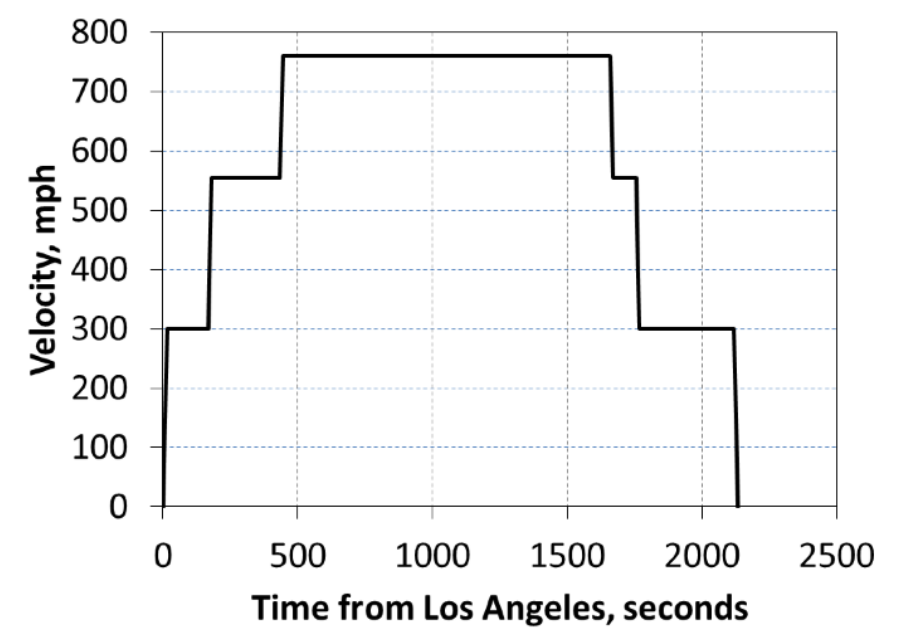
\includegraphics[scale=0.27]{figs/hyperloop.png}
\caption{Izquierda: figura para el problema 1. Derecha: figura para el
  problema 3.}
\end{center}
\end{figure}
{\bf NOTA}: Todas las respuestas deben tener una justificaci\'on
f\'isica y matem\'atica adecuada. Tome $g=10$ m/s$^{2}$. 100 puntos
corresponden a una calificaci\'on de 5.0.
\end{document}
